\chapter{Einführung}

\label{chap:intro}

Das Hidden Markov Model hat im Bereich des machinellen Lernens viele Anwendungsfälle. In der vorgelegten Arbeit wird die Funktionsweise des Hidden Markov Model erklärt werden (Kapitel \ref{mainsec:hmm}). Die dafür notwendigen Grundlagen werden in den nachfolgenden Abschnitten und im Kapitel \ref{mainsec:mk} beleuchtet.
Kapitel \ref{mainsec:result} befasst sich mit einer Einschätzung des Hidden Markov Models und dem Vergleich mit anderen Ansätzen im Machine Learning Kontext.

\section{Machine Learning}
Machine Learning befasst sich mit der modellierung des Lernvorgangs auf einem Computer \cite{marsland}. Es wird versucht ein ``künstliche'' Generierung von Wissen aus Erfahrung zu erzeugen.
Dabei wird anhand von Beispielen ``gelernt'', sodass nicht nur die selben Daten wieder erkannt werden können, sondern auch ähnliche bzw. unbekannte Daten klassifiziert werden. Diese Transferleistung nennt man Generalisierung und ist auch beim Menschen eine wichtige Eigenschaft im Lernvorgang.

So können wir Äpfel von Birnen (Siehe Abbildung \ref{fig:apfelbirne} \footnote{Quelle: \url{http://www.lifeline.de/img/abnehmen/origs76797/7656955923-w830-h830/Birne-und-Apfel.jpg}}) unterscheiden, egal, ob wir genau diese Frucht schon einmal gesehen haben. Wir entscheiden anhand gelernter Merkmale, um welche Frucht es sich vermutlich handelt. Merkmale sind bspw. Größe, Form, Farbe, Geruch etc.

\begin{figure}[htbp] \centering
    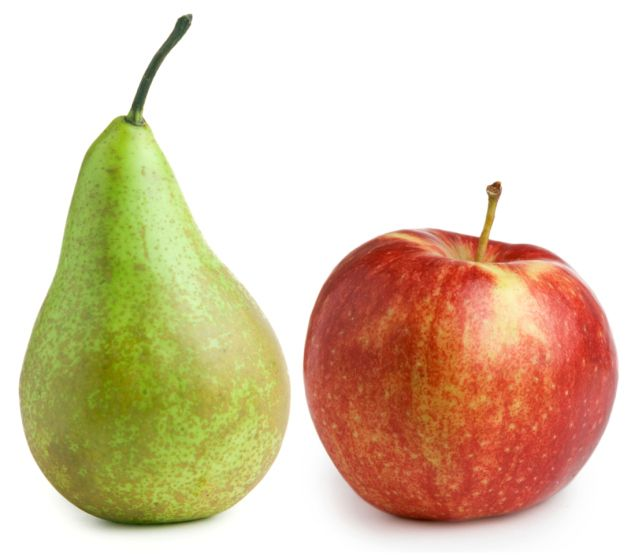
\includegraphics[width=0.25\textwidth]{Bilder/Kap1/birneapfel}
    \caption{ Birne und Apfel unterscheiden sich durch Farbe, Form etc. - einen Stiel haben jedoch beide}
    \label{fig:apfelbirne}
\end{figure}


Die Extraktion signifikanter Merkmale ist ein wichtiger Teil von Machine Learning. Viele Eigenschaften eines Objektes sind nicht geeignet es von anderen zu unterscheiden. Im Apfel-Birnen-Beispiel würde das Merkmal ``Stiel'' nicht zu einer Unterscheidung führen.

Der nächste Schritt ist das Training des Systems. Hierbei wird zwischen drei algorithmischen Ansätzen unterschieden:
\begin{itemize}
\item Überwachtes Lernen
\item Unüberwachtes Lernen
\item Bestärkendes Lernen
\end{itemize}
Die häufigste menschliche Lernform, ist das bestärkende Lernen, hier wird mit ``Belohnung'' und ``Bestrafung'' gearbeitet. 
Im Machine Learning Bereich ist jedoch Überwachtes und Unüberwachtes Lernen sehr viel häufiger zu finden. Beim überwachten Lernen, werden mehrere Eingaben und Lösungen an den Algorithmus überreicht und nach einigen Durchgängen sollte er in der Lage  sein Assoziationen herzustellen. Je nach Algorithmus werden hierzu Funktionen und Gewichtungen angepasst. 

Das Hidden Markov Model ist im Bereich des Unüberwachten Lernens beheimatet. Aus der Menge der Eingaben wird ein Modell erzeugt, das Vorhersagen ermöglichen soll. Mit einem Expectation-Maximization-Algorithmus (EM-Algorithmus) wird versucht, die vorliegenden Daten in Kategorien einzuteilen, sodass die Daten optimal erklärt werden. Eine Form des EM-Algorithmus kommt auch beim Hidden Markov Model zum Einsatz.

Weitere Machine Learning Ansätze sind 
\begin{itemize}
\item Neuronale Netze
\item Support Vector Machine
\item K-Means
\end{itemize} 

\begin{figure}[htbp] \centering
    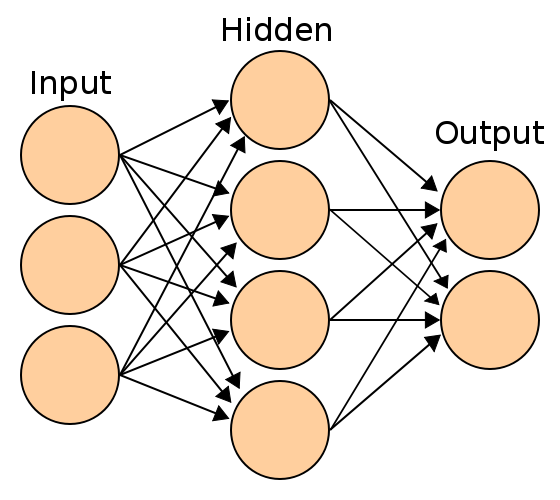
\includegraphics[width=0.4\textwidth]{Bilder/Kap1/neuralnetwork}
    \caption{ Vereinfachte Darstellung eines neuronalen Netzwerkes mit 3 Merkmaldimensionen. }
    \label{fig:neural}
\end{figure}

Neuronale Netze versuchen das menschliche Gehirn mit seinen Neuronen und Synapsen nachzubauen \cite{neuron}. Für jede Dimension des Merkmalsvektors sind Neuronen vorhanden, welche wiederum mit anderen Neuronen verschaltet sind. Beim Training werden die Gewichtungen der einzelnen Verschaltungen verändert.
Abbildung \ref{fig:neural} \footnote{Quelle: \url{http://en.wikipedia.org/wiki/Artificial_neural_network\#/media/File:Artificial_neural_network.svg}} zeigt ein vereinfachtes neuronales Netz mit drei Inputs, vier weiteren Neuronen und zwei Outputs.

\begin{figure}[htbp] \centering
    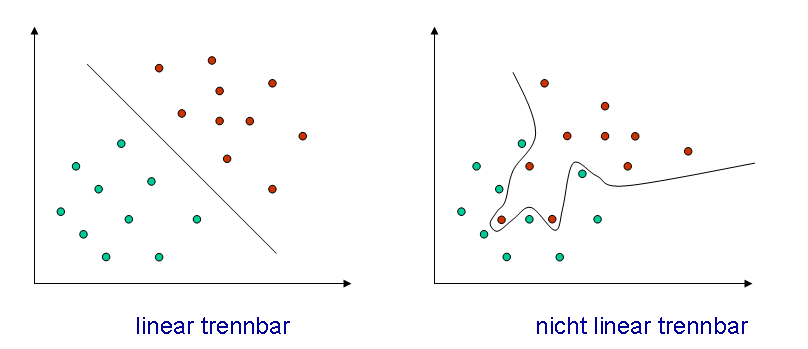
\includegraphics[width=0.5\textwidth]{Bilder/Kap1/svm}
    \caption{ Daten lassen sich nicht immer linear trennen.}
    \label{fig:svm}
\end{figure}

Die Support Vector Machine (Stützvektormaschine) versucht die Daten durch lineare Trennung zu Klassifizieren (Siehe Abbildung \ref{fig:svm} \footnote{Quelle: \url{http://upload.wikimedia.org/wikipedia/de/a/a0/Diskriminanzfunktion.png}})
\cite{svm}. Es wird versucht, den Stützvektor möglichst weit von den beiden Klassen entfernt zu erstellen (Large-Margin-Classifier).


Im Abschnitt \ref{sec:compare} werden die vorgestellten Ansätze mit dem Hidden Markov Model verglichen.



\section{Mathematische Grundlagen}
Im folgenden Abschnitt werden grundlegende mathematische Grundlagen und Definition vorgestellt.

\subsection{Zeit-diskreter Prozess}
\label{sec:timedisc}
Ein zeit-diskreter Prozess beschreibt die Eigenschaft, dass sich die Zustände eines Systems immer im selben zeitlichen Abstand ändern (Äquidistante Zeitabstände). Beispielsweise wird jede Sekunde ein Tick ausgelöst, welcher zu einer Zustandsänderung führt. 
Ist dies nicht der Fall, dann spricht man von einem zeit-kontinuierlichen Prozess.

\subsection{Wahrscheinlichkeit}
\label{sec:prop}
Die Wahrscheinlichkeit (Probabilität) beschäftigt sich mit der mathematischen Untersuchung von Zufallsgeschehen. Gemeinsam mit der  Statistik, bildet sie das mathematische Teilgebiet der Stochastik.

Dafür wird von einem Zufallsexperiment ausgegangen und dieses analysiert. Alle möglichen Ergebnisse dieses Experiments werden in der Ergebnismenge $\Omega$ zusammengefasst. Meistens ist nicht das genaue Ergebnis $\omega \in \Omega$ von Interesse, sondern lediglich, ob das Ergebnis in einer bestimmten Teilmenge von $\Omega$ liegt. Weiterhin wird mit dem Ereignisraum $\Sigma$ definiert und enthält alle möglichen Ereignisse. Die Wahrscheinlichkeit wird mit $P$ bezeichnet und bewegt sich im Intervall $[0, 1]$. 

Im Beispiel ``Münzwurf'' ergeben sich dann folgende Definitionen \footnote{Quelle: \url{http://de.wikipedia.org/wiki/Wahrscheinlichkeitstheorie}}.

\begin{itemize}
\item Ergebnismenge $\Omega = \{Zahl, Kopf\}$
\item Ereignisraum $\Sigma = \{\emptyset, \{Zahl\}, \{Kopf\}, \Omega\}$
\item Wahrscheinlichkeiten
	\begin{itemize}
	\item $P(\emptyset) = 0$
	\item $P(\{Zahl\}) = 1 - P(\{Kopf\})$
	\item $P(\Omega) = 1$
	\end{itemize}
\end{itemize}
Bei den Wahrscheinlichkeiten ist $P(\emptyset) = 0$ und $P(\Omega) = 1$, da es ein Ergbenis geben muss und dieses aus $\Omega$ stammen muss. Die Wahrscheinlichkeit von $\{Zahl\}$ und $\{Kopf\}$ addieren sich zu 1. Bei einer fairen idealen Münze haben Kopf und Zahl jeweils eine Wahrscheinlichkeit von 0.5 (50\%).


\subsection{Bedingte Wahrscheinlichkeit}
\label{sec:condprop}
Die bedingte Wahrscheinlichkeit beschreibt die Wahrscheinlichekit für ein das Eintreten eines Ereignisses $A$ unter der Bedingung, dass vorher ein Ereigniss $B$ eingetreten ist. $P(A | B)$ drückt diesen Zusammenhang aus, der $|$ ist als ``unter der Bedingung'' zu lesen.
\begin{equation}
\label{equ:transprop}
P(A | B) = \frac{P(A \cap B)}{P(B)}
\end{equation}
Definition \ref{equ:transprop} zeigt eine weitere Schreibweise der bedingten Wahrscheinlichkeit, bei der die Wahrscheinlichkeit, dass $A$ und $B$ gemeinsam auftreten, durch die Wahrscheinlichkeit, dass $B$ eintritt geteilt wird.





